\subsection{Calibration Frame Preparation}

For each camera location of the dataset, a set of calibration frames (generally fifteen,
location dependant) and corresponding binary masks were prepared.
The frames were extracted from location-specific reference videos supplied with the dataset
consisting of a person standing, facing the camera, at known distance intervals
and holding a sheet of A4 paper labelled with the corresponding distance.

\subsubsection{Frame Extraction}
In an effort to streamline the frame extraction process, an extractor program was created
(Figure~\ref{fig:frame_extractor}).
This tool enabled reference videos to be dragged and dropped into a GUI window allowing for the
easy navigation between individual frames to extract the optimal one for each distance.
With this software, the next/previous frames are accessed with the 'left'/'right' arrow keys, the frame
index position is moved ahead/behind 20 places with the 'd'/'a' keys and the frame found at a specific
timestamp is accessed with the 's' key followed by entering a time (in seconds) into an input bar.
The active frame (at the current index) can be saved to disk with the 'enter' key followed by entering
a filename in an input bar.
\vspace{5mm}

\begin{figure}[htbp]
    \centering
    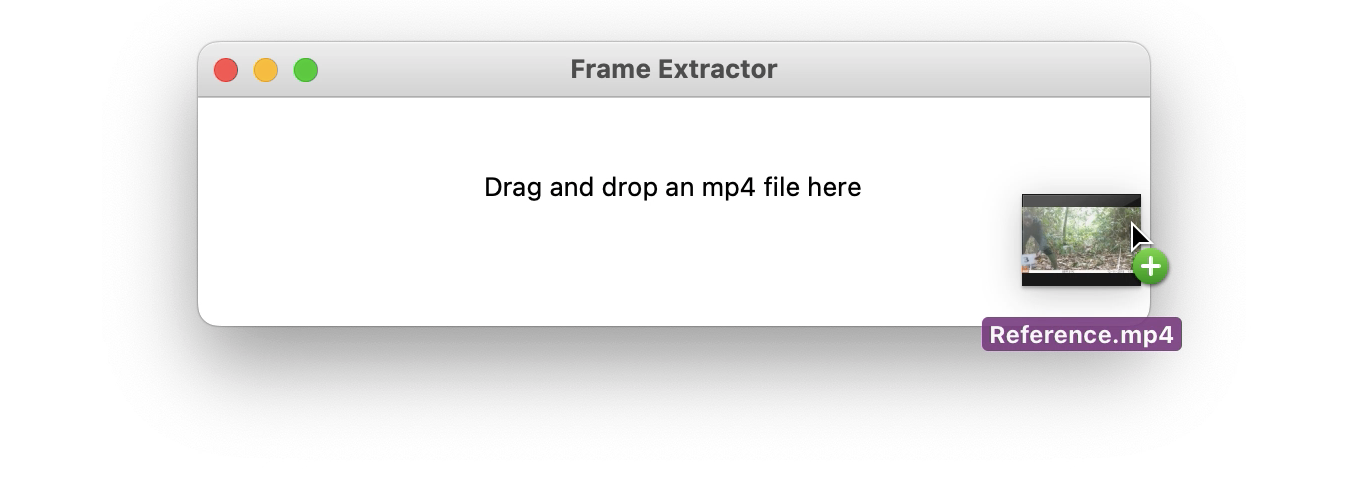
\includegraphics[scale=0.5]{body/experimental/assets/frame_extractor/drag_drop}
    \vspace{-3mm}
    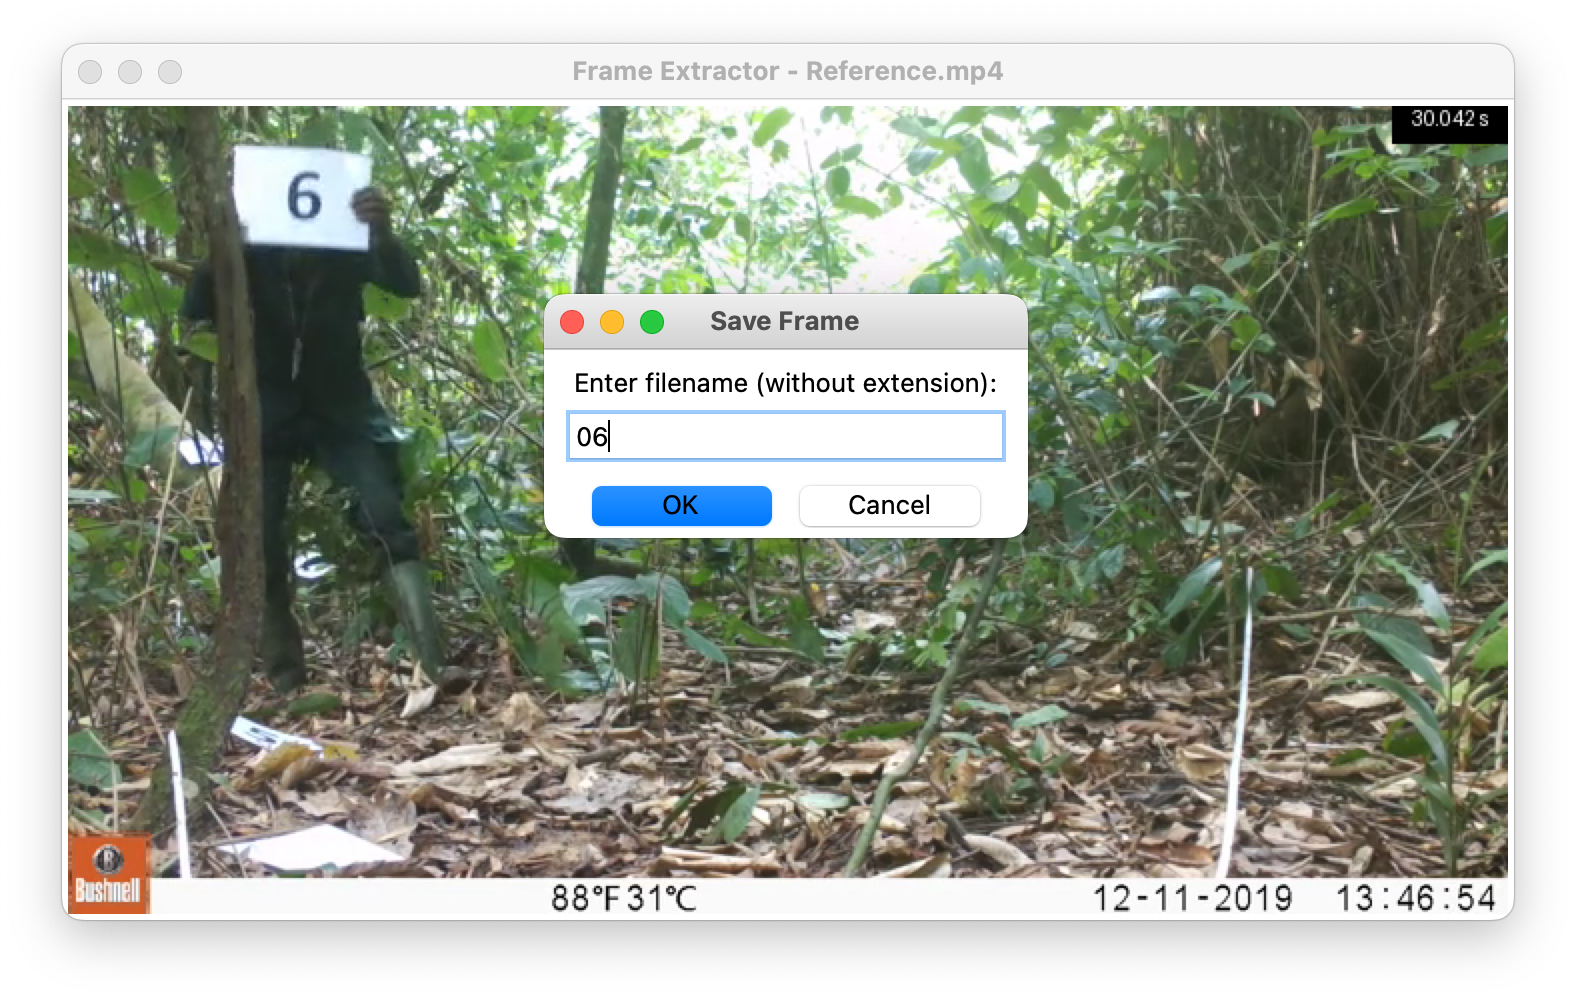
\includegraphics[scale=0.5]{body/experimental/assets/frame_extractor/save_frame}
    \caption{Frame extractor program showing the drag/drop (top) and save frame (bottom) features}
    \label{fig:frame_extractor}
\end{figure}

\clearpage

The

\subsubsection{Frame Mask Creation}
Mask creation using GIMP, potential use of segment anything